\chapter{Opis projektnog zadatka}
		
		\indent Cilj ovog projekta je razviti programsku podršku za stvaranje web aplikacije \emph{"Iznajmi Romobil"} koja će korisniku omogućiti da iznajmi vlastiti romobil u vrijeme kada ga ne koristi, a korisnicima koji ne posjeduju romobil daje mogućnost najma romobila. \newline
		\indent Prilikom pokretanja aplikacije prikazuje se glavna stranica s oglasima za najam romobila. Neprijavljen korisnik oglase može samo pregledavati, dok prijavljen korisnik može i stupiti u kontakt s iznajmljivačem te u konačnici i unajmiti odabrani romobil. \\
		\indent Ako korisnik nema izrađen račun u aplikaciji, ima mogućnost registracije. Prilikom registracije, korisnik unosi:
		\begin{packed_item} 
			\item {ime}
			\item {prezime}
			\item {nadimak}
			\item {email adresa}
			\item {broj kartice}
			\item {lozinka}
			\item {kopija osobne iskaznice}
			\item {potvrda o nekažnjavanju}  
		\end{packed_item}
		\indent Tijekom obrade registracije na strani poslužitelja korisniku se dodjeljuju ovlasti. S obzirom na to da korisnik može biti i iznajmljivač i klijent, jedna će ovlast  objediniti te uloge. Također, sustav razlikuje i ovlast admin.  \\
		\indent Jednom kada se korisnik registrira, ili je već prije izradio račun, ima mogućnost prijave u aplikaciju. Prilikom prijave korisnik unosi korisničko ime i lozinku. Jednom kada potvrdi prijavu, na poslužiteljsku stranu šalju se uneseni podaci, a povratno poslužitelj odgovara ili s greškom ili s JSON web tokenom u kojem su spremljeni ime i prezime korisnika te njegove ovlasti. \\
		\indent Ako je prijava uspješno provedena korisnika se prosljeđuje na početnu stranicu. Kao što je prethodno navedeno, prijavljeni korisnik sada može iznajmljivati i unajmljivati romobile. Prijavljeni korisnik može pregledavati i mijenjati svoje osobne podatke. Dodatno mu je omogućeno i postavljanje profilne slike.\\
		\indent Da bi iznajmljivač postavio svoj romobil na iznajmljivanje mora ga registrirat. Prilikom registracije romobila iznajmljivač unosi slike romobila kao dokaz trenutnog stanja. Jednom kada je romobil registriran, iznajmljivač postavlja ponude za iznajmljivanje te za svaku unosi:
		\begin{packed_item} 
			\item trenutna lokacija romobila
			\item lokacija povratka romobila
			\item vrijeme povratka romobila
			\item cijena iznajmljivanja po prijeđenom kilometru
			\item iznos novčane kazne u slučaju da romobil ne bude vraćen na vrijeme
		\end{packed_item}
		Iznajmljivač svoju ponudu može objaviti i na društvenoj mreži Facebook.\\
		\indent Klijent pretražuje oglase i kada se odluči za romobil, može se javiti iznajmljivaču. Komunikacija između klijenta i iznajmljivača odvija se preko poruka putem aplikacije. Iznajmljivač i klijent mogu se detaljnije dogovoriti oko vremena i lokacije preuzimanja romobila. Kada klijent pošalje poruku iznajmljivači, iznajmljivač dobiva obavijest. Ako stvarno stanje romobila kojeg klijent preuzme ne odgovara stanju kakvo je prikazano na slikama, klijent može stare slike romobila zamijeniti vlastitim. Također, može i dati kratki opis razlika između starih slika i stvarnog stanja. Ako iznajmljivač smatra da zamjena slika nije utemeljena, tu zamjenu može prijaviti administratoru. Klijent je dužan vratiti romobil u zadano vrijeme i lokaciju povratka, u suprotnom će mu biti izrečena novčana kazna.  \\
		\indent Admin je korisnik najveće razine te on ima mogućnost pregleda svih korisnika i može ih brisati. Admin pregledava prijave iznajmljivača i odlučuje hoće li se zamjena slika izvršiti i li ne. Ako administrator prihvati prijavi iznajmljivača, slike romobila se vraćaju na one koje su bile prije klijentove izmjene. Njegova odluka dolazi kao obavijest klijentu i iznajmljivaču. Također, admin pregledava dostavljenu kopiju osobne iskaznice i potvrdu o nekažnjavanju. Ako uspostavi da su dokumenti neispravni, može trajno ukloniti korisnika s aplikacije.\\
		\indent Svaki romobil mora imat mjerač prijeđenih kilometara te on mora bit povezan s aplikacijom kako bi se znalo koliko je kilometara prešao klijent. Kada istekne vrijeme povratka iznajmljivač dobiva obavijest u aplikaciji u kojoj je navedeno koliko je kilometara klijent prešao. Klijent također dobiva obavijest u kojoj su napisani detalji transakcije. \\
		\indent Nakon što je iznajmljivanje završeno, iznajmljivač može ocijeniti klijenta i napisati komentar. Ocjene i komentari su vidljivi na profilima korisnika. \\
		\indent Korisnik na svom profilu može pregledati podatke o prethodnim vožnjama, ili ako se radi o iznajmljivaču podatke o prethodnim najmovima romobila.\\ \\
		
		\indent Korist ovog projekta je omogućiti ljudima jednostavan pristup električnim romobilima. Kvalitetan električni romobil je mnogima preskup, tako da oni koji ga ne posjeduju mogu lako i brzo iznajmiti romobil na dane kada im je potreban. Ljudi koji ne koriste svoj romobil, a ne žele da propada u skladištu, mogu ga iznajmiti drugima i na taj način ostvariti dodatan prihod. \\
		\indent U urbanim sredinama gužve u prometu postaju sveprisutni problem koji otežava svakodnevno kretanje i troši vrijeme. U takvim okolnostima, ljudi traže alternativne metode prijevoza koje su brže, praktičnije i održive. I tu vidimo priliku za našu aplikaciju.\\
		
		\indent Aplikacija bi mogla biti unaprijeđena tako da klijent ima veću mogućnost filtriranja prikazanih oglasa. Na primjer može pretraživati oglase samo u okolici njegove lokacije ili romobile koji zadovoljavaju njegove zahtjeve, na primjer da maksimalna brzina romobila nije manja od 45 km/h ili prema dometu romobila. Također, moguće je aplikaciju učiniti profitabilnijom za vlasnika aplikacije.
		Na primer vlasnik bi mogao od svake transakcije dobit određeni postotak. Druga mogućnost bi bila da iznajmljivači moraju plaćati mjesečnu pretplatu kako bi mogli dat svoje romobile u najam. \\
		
		\indent Tvrtka Bolt, koja je u hrvatskoj prepoznatljiva po uslugama dostave hrane i prijevoza, u pojedinim gradovima nudi mogućnost najma romobila. Pa se tako u glavnom gradu Belgije, Briselu, romobili spremni za najam mogu pronaći gotovo u svakoj ulici. Potrebno je imati novčana sredstva u Bolt aplikaciji, na romobilu se skenira QR kod i spremni ste za vožnju. Cijena se također obračunava po prijeđenom kilometru. A jednom kada ste gotovi odjavite se s romobila, romobil se zaključa i spreman je za idućeg korisnika, a Vama se 	automatski provede transakcija.
		
		\begin{figure}[h]
			\centering
			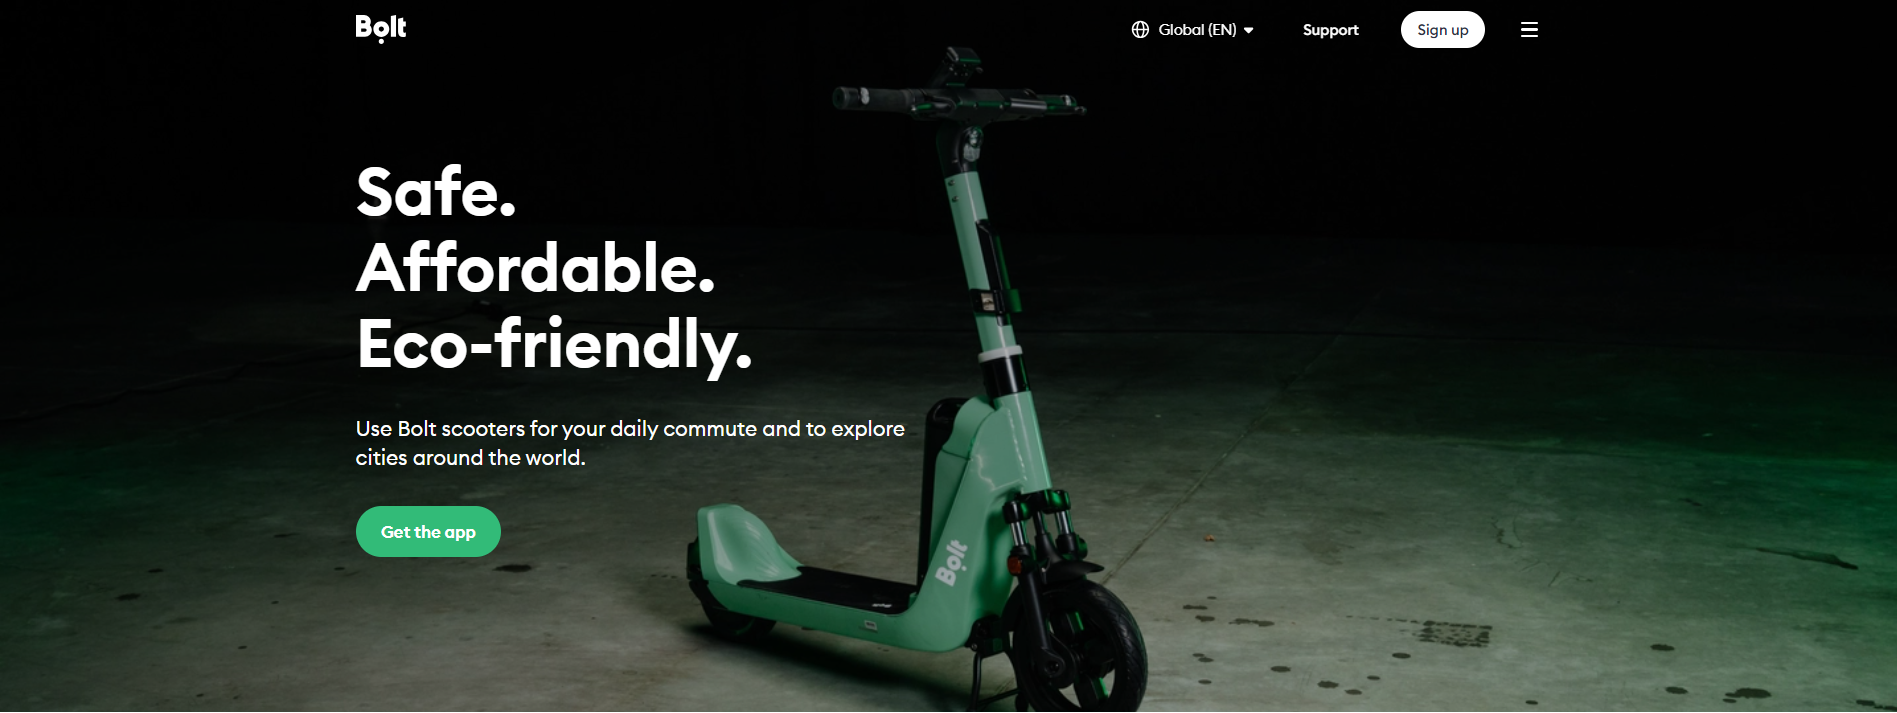
\includegraphics[width=0.8\textwidth]{slike/bolt-1.png}
			\caption{Početna stranica za najam rombila tvrtke Bolt}
			\label{fig:bolt-1}
		\end{figure}
		
		\begin{figure}[t]
			\centering
			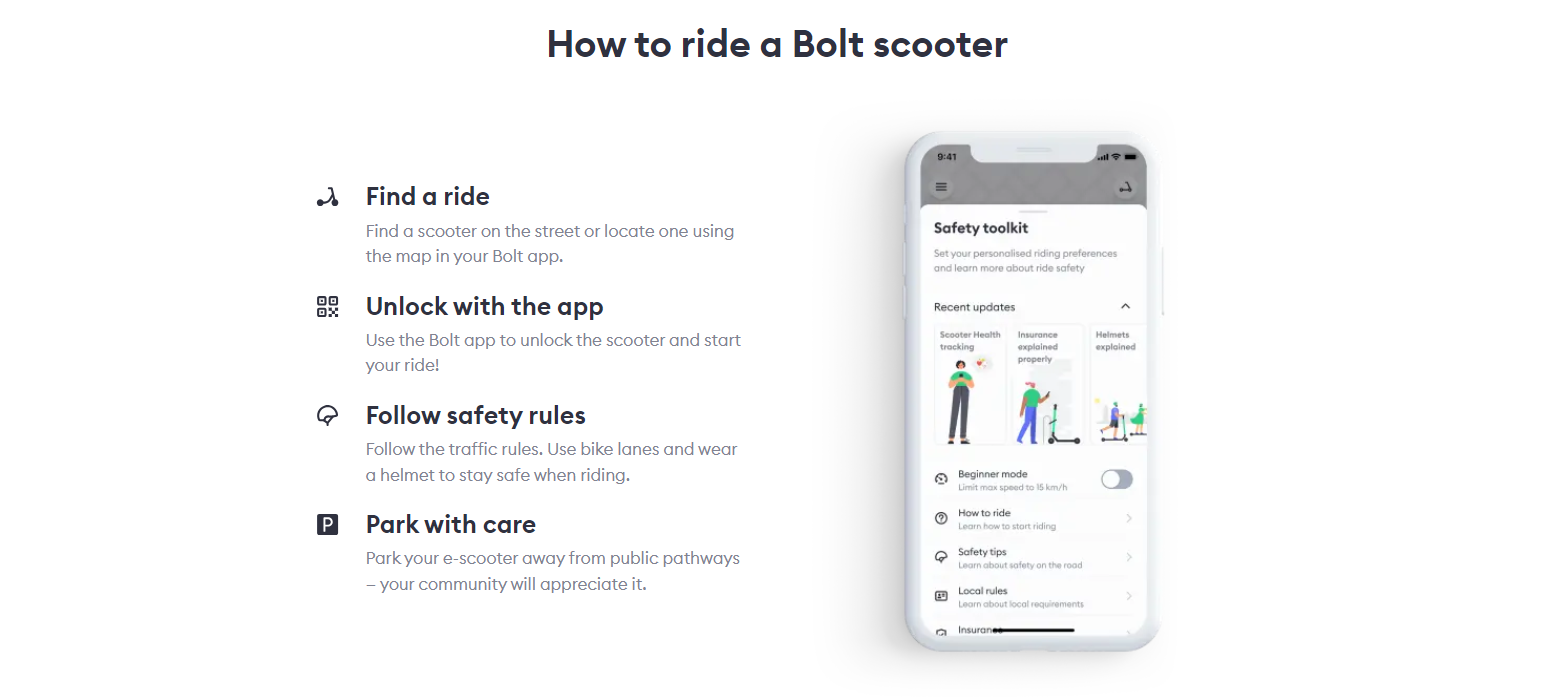
\includegraphics[width=0.8\textwidth]{slike/bolt-2.png}
			\caption{Instrukcije za korištenje romobila tvrtke Bolt}
			\label{fig:bolt-2}
		\end{figure}
		
		\indent Aplikacija Fat LIama nudi mogućnost najma električnih romobila diljem svijeta. Razlikuje se po tome što je cijena iskazana po danu najma. Korisnik može odabrati lokaciju, pretražuje ponuđene oglase te ima mogućnost najma na više dana.\\
		
		\begin{figure}[t]
			\centering
			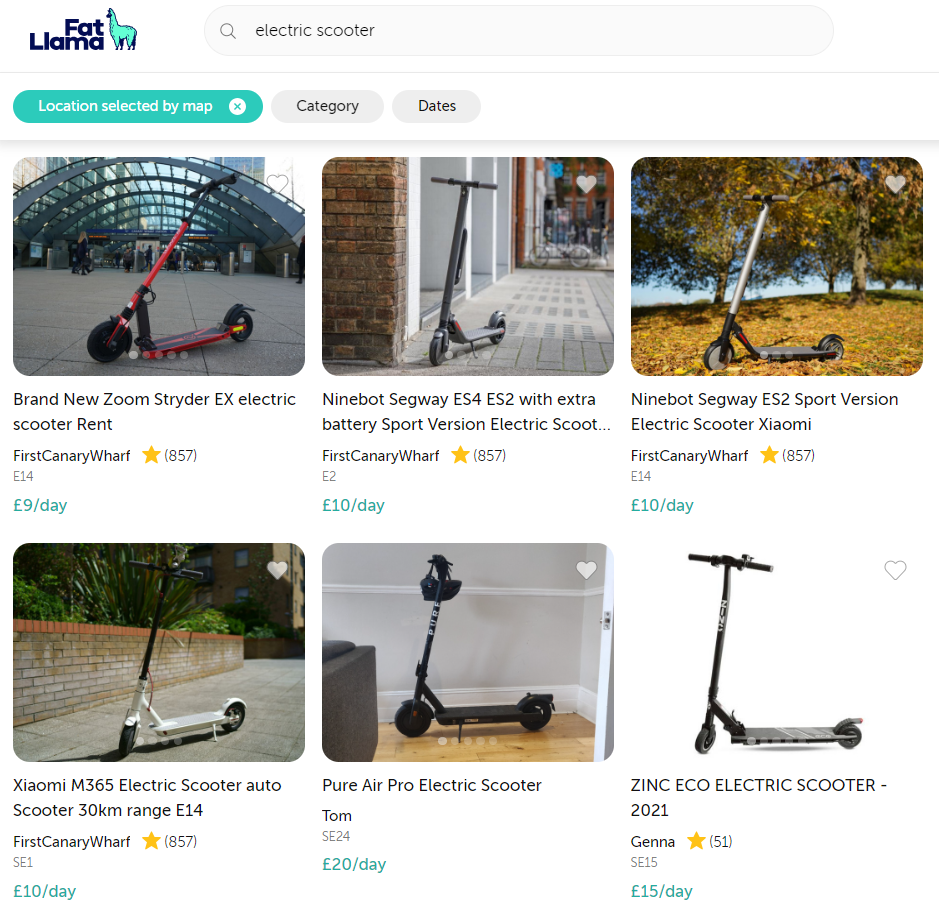
\includegraphics[width=0.8\textwidth]{slike/fat-liam.png}
			\caption{Najam romobila Fat LIama}
			\label{fig:fat-liama}
		\end{figure}
		
		
		\indent Aplikacija Fat LIama nudi mogućnost najma električnih romobila diljem svijeta. Razlikuje se po tome što je cijena iskazana po danu najma. Korisnik može odabrati lokaciju, pretražuje ponuđene oglase te ima mogućnost najma na više dana.\\
		
		
		
		
	